\section{Zielsetzung}
\label{sec:Zielsetzung}
Als Ziel dieses Versuchs sollen mithilfe des Photoeffekts die Zusammenhänge zwischen der Frequenz
des Lichts und der Energie der Elektronen, sowie die Abhängigkeit des resultierenden
Photostroms von der Stärke des angelegten Gegenfeldes untersucht werden.
\section{Theorie}
\label{sec:Theorie}
\subsection{Grundsätzliche Prinzip des Photoeffekts}
\label{Grundsätzliche_theo}
Licht hat zwei unterschiedliche Erscheinungsformen. Zum einen das Wellenmodell,
welches Phänomene wie Interferenz und Beugung erklärt und zum anderen das Korpuskelmodell oder
auch das Teilchenmodell, womit sich der Compton-Effekt, die Paarbildung und der Photoeffekt erklären lassen.\\
Für diesen Versuch wird das Korpuskelmodell benutzt, weil die Wechselwirkung von Photonen mit Materie untersucht wird.
Der grundlegende Aufbau zur Messung des Photoeffektes ist in \autoref{fig:Abb_1} dargestellt.
\begin{figure}[H]
    \centering
    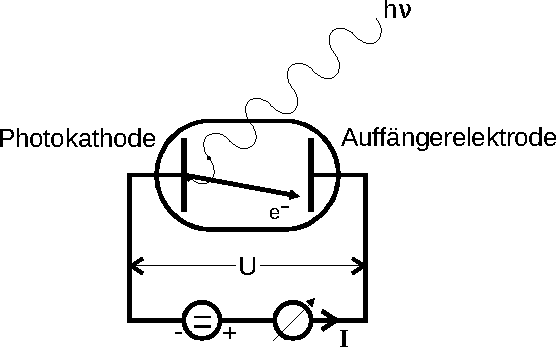
\includegraphics[width=0.3\textwidth]{build/Abb_1.pdf}
    \caption{Grundlegender Aufbau zur Messung des Photoeffektes.\cite{V500}}
    \label{fig:Abb_1}
\end{figure}
Eine negativ geladene Photokathode wird im Vakuum mit monochromatischem Licht aus einer Quelle bestrahlt.
Laut dem Teilchenmodell besteht Licht aus Photonen, auch Lichtquanten genannt, welche ein diskretes
Energiespektrum besitzen. Wenn diese Energie $E_{Ph}$ groß genug ist, können Photonen beim Auftreffen auf die Photokathode
Elektronen aus dem Material der Photokathode herauslösen.
Wenn die Energie größer als die Austrittsarbeit $A_K$ des Elektrons ist, wird die restliche Energie übertragen 
und in kinetische Energie $E_{kin}$ der Elektronen umgewandelt.
\begin{equation}
    E_{Ph} = h\nu = A_K + E_{kin}
    \label{eqn:Energie}
\end{equation}
$h$ ist das Plank'sche Wirkungsquantum und es gilt
\begin{equation}
    \nu = \frac{c}{\lambda}
    \label{eqn:Frequenz}
\end{equation}
als Zusammenhang zwischen der Frequenz $\nu$ und der Wellenlänge $\lambda$.\\
Die Elektronen bewegen sich zu einer positiven Anode, an welcher der Strom der herausgelösten
Elektronen als Photonenstrom gemessen wird. Es existiert eine Grenzfrequenz, da keine Elektronen 
ausgelöst werden bei $E_{Ph} < A_K$. Außerdem ist die Lichtintensität proportional zur Anzahl der 
Photonen pro Zeit- und der Raumwinkel und pro Photon kan nur ein Elektron ausgelöst werden.
Daraus folgt, dass die Anzahl der pro Zeit herausgelösten Elektronen proportional zur Lichtintensität ist.
Aus \autoref{eqn:Energie} folgt, dass die kinetische Enrgie der Elektronen abhängig von der Frequenz $\nu$ des
Lichtes ist, mit der die Photokathode bestrahlt wird.

\subsection{Experimentelle Messung des Photoeffektes mit der Gegenfeldmethode}
\label{sec:Gegenfeldmethode}
Die Gegenfeldmethode wird dazu verwendet den Photoeffekt zu untersuchen. Dabei wird ein variables Potential $U$
zwischen Photokathode und Anode angelegt. Dies führt dazu, dass der gemessene Photostrom kleiner wird, weil nur noch Elektronen 
die Anode erreichen, dessen Energie ausreicht um das Feld zu überwinden. Der Photostrom verschwindet, wenn
\begin{equation*}
    e U_g = \frac{1}{2} m_0 v^2_{max}
\end{equation*}
gilt, also auch die Elektronen mit der größten Geschwindigkeit $v_{max}$ bei einer Grenzgegenspannung $U_g$ die Kathode nicht mehr erreichen.
Die Elementarladung wird als $e$ dargestellt und die Ruhemasse als $m_0$. Mit dem Gegenfeld muss die Energiebilanz aus \autoref{eqn:Energie} geändert werden.
Die übertragene Energie teilt sich in Austrittsarbeit $A_K$ und Arbeit des Gegenfeld $E_{kin} \geq e U_g$ auf.
\begin{equation}
    E_{Ph} = h \nu = A_K + e U_g
\end{equation}
Der Photonenstrom fällt bei steigender Gegenspannung $U$ nicht sofort ab, was in \autoref{fig:Abb_2} dargestellt ist.
\begin{figure}[H]
    \centering
    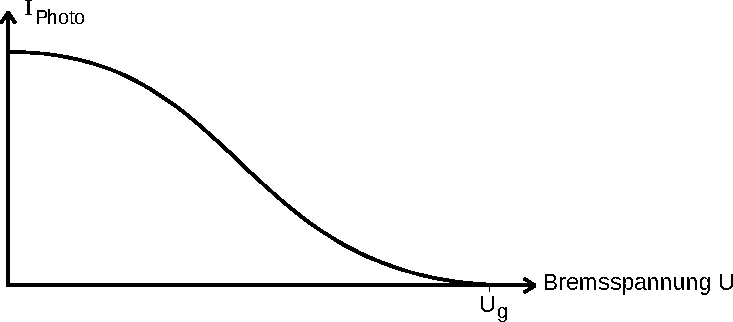
\includegraphics[width=0.3\textwidth]{build/Abb_5.pdf}
    \caption{Verlauf des Photostroms bei steigender Gegenspannung.\cite{V500}}
    \label{fig:Abb_5}
\end{figure}
Der Grund für diese Kurve ist, dass die Elektronen im Material verschiedene Energieniveaus besitzen 
und daher verschiedenenergetisch sind, wenn sie aus der Photokathode herausgelöst werden.\\
Die Energieverteilung kann mit der Fermi-Dirac-Statistik erläutert werden, welche besagt, das sich die Elektronen auf einem Intervall
von 0 bis zu einer Fermi-Energie $\zeta$ beschreiben lässt. Die obere Grenze $\zeta$ ist dabei materialabhängig.
Für den Photonenstrom ergibt sich der Zusammenhang
\begin{equation}
    I_{Ph} \propto U^2,
\end{equation}
weil die herausgelösten Elektronen teilweise eine Energie haben, die größer als $h\nu -A_K$ ist.
In \autoref{fig:Abb_5} ist die Wurzel des Photonenstroms gegen die Spannung aufgetragen, wobei die Nullstelle  die 
Grenzfrequenz bildet.
Bei kleinen Wellenlängen muss eine Beschleunigungsspannung $U_b$ angelegt werden, damit ein Photostrom entsteht und
\begin{equation*}
    h\nu + e U_b \geq A_A
\end{equation*}
gilt. Die Energie der Elektronen muss größer als die Austrittsarbeit $A_A$ der Anode sein, damit die Elektronen auf die Anode treffen.
Dabei setzt sich die Energie der Elektronen aus $E = h \nu $ und der elektrischen Energie $e U_b$ zusammen.

